\section{Trabajo Extra: Diseño UX y Validación con Usuarios}

En cumplimiento del numeral 6 de la guía de laboratorio (\textit{Trabajo extra: Mejorar diseño UX y validar con usuarios}), se implementaron optimizaciones heurísticas y se capturaron evidencias directas de la experiencia de usuario sobre el sistema \textbf{SIGC-CUSCO} en funcionamiento.

\subsection{Heurísticas de Usabilidad Aplicadas}
\begin{itemize}[nosep]
    \item \textbf{Visibilidad del Estado del Sistema:} Badges de estado dinámicos (\textit{Abierto}, \textit{En curso}, \textit{Concluido}), contadores de vacantes disponibles en tiempo real y confirmaciones visuales tipo \textit{toast} mediante la librería \texttt{vue-sonner}.
    \item \textbf{Correspondencia entre el Sistema y el Mundo Real:} Uso de terminología académica formal (actas de notas, horas pedagógicas, escala vigesimal 0--20) y validación de documentos oficiales del Perú (DNI de 8 dígitos).
    \item \textbf{Control y Libertad para el Usuario:} Filtros ágiles de búsqueda sin recarga forzada, vistas diferenciadas por rol (Administrador, Docente, Participante) y navegación reactiva mediante Inertia.js.
    \item \textbf{Prevención y Recuperación de Errores:} Mensajes contextuales claros, bloqueo automático de inscripción al agotarse cupos y validación criptográfica ante códigos de certificado inexistentes.
\end{itemize}

\subsection{Evidencias de la Experiencia de Usuario (UX) en el Sistema Real}
Las Figuras \ref{fig:real_dashboard_ux}, \ref{fig:real_welcome_ux} y \ref{fig:real_course_ux} evidencian la implementación UX en la aplicación web funcional:

\begin{figure}[H]
    \centering
    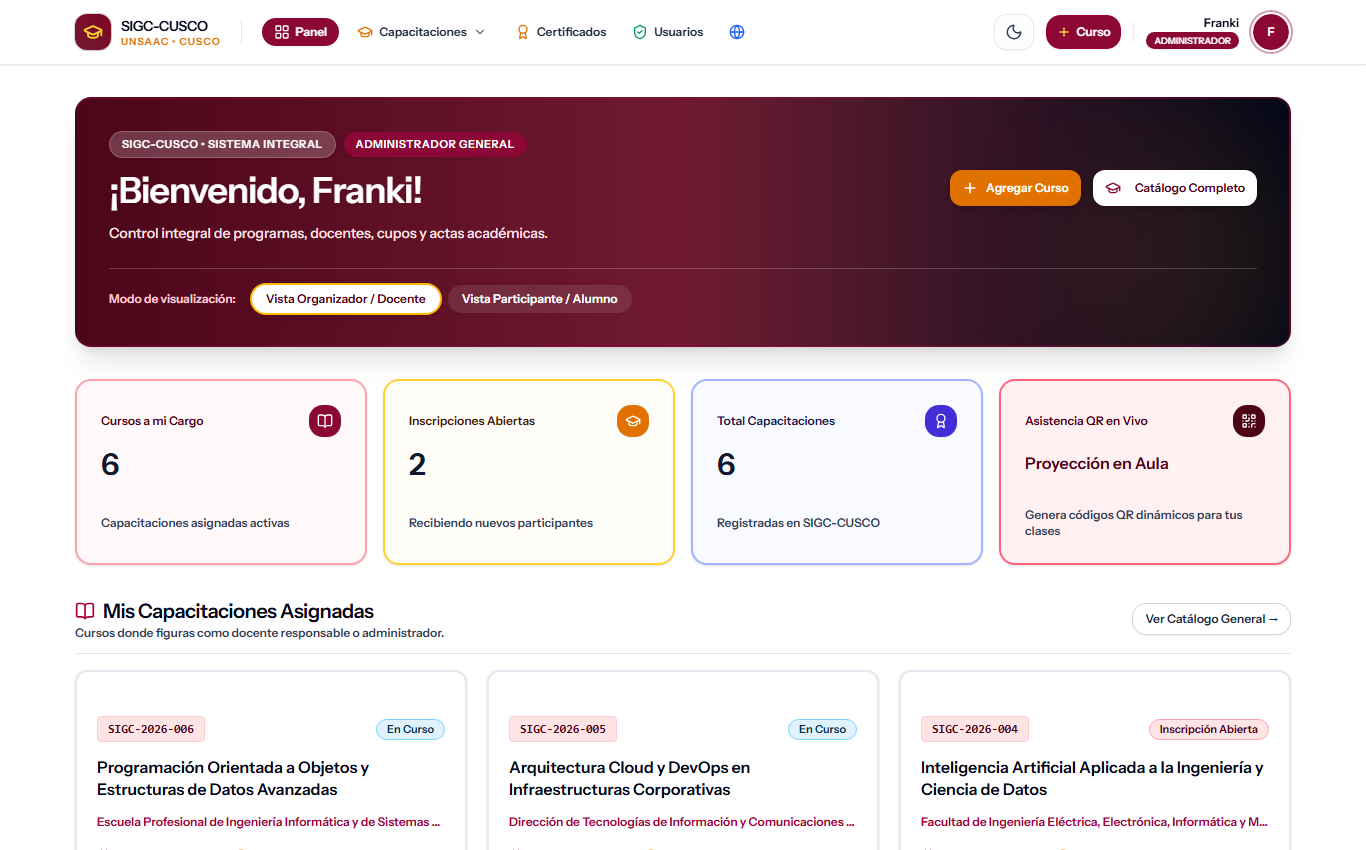
\includegraphics[width=0.94\textwidth]{sigc_real_dashboard.png}
    \caption{Panel Principal (Dashboard) Autenticado: Métricas de cursos, accesos rápidos y estado académico.}
    \label{fig:real_dashboard_ux}
\end{figure}

\begin{figure}[H]
    \centering
    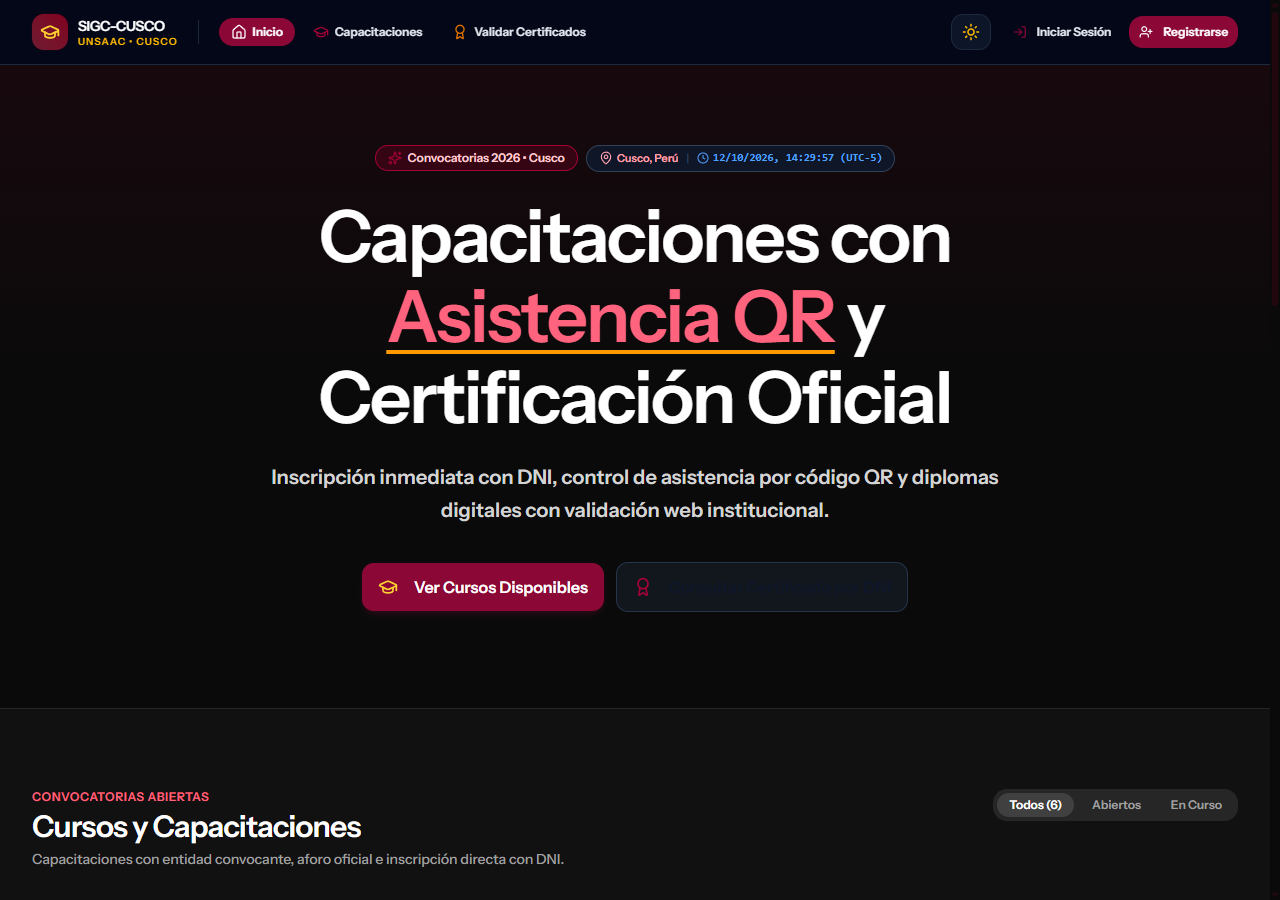
\includegraphics[width=0.94\textwidth]{sigc_real_welcome.png}
    \caption{Portal Público de Inicio: Catálogo interactivo de cursos y convocatorias abiertas.}
    \label{fig:real_welcome_ux}
\end{figure}

\begin{figure}[H]
    \centering
    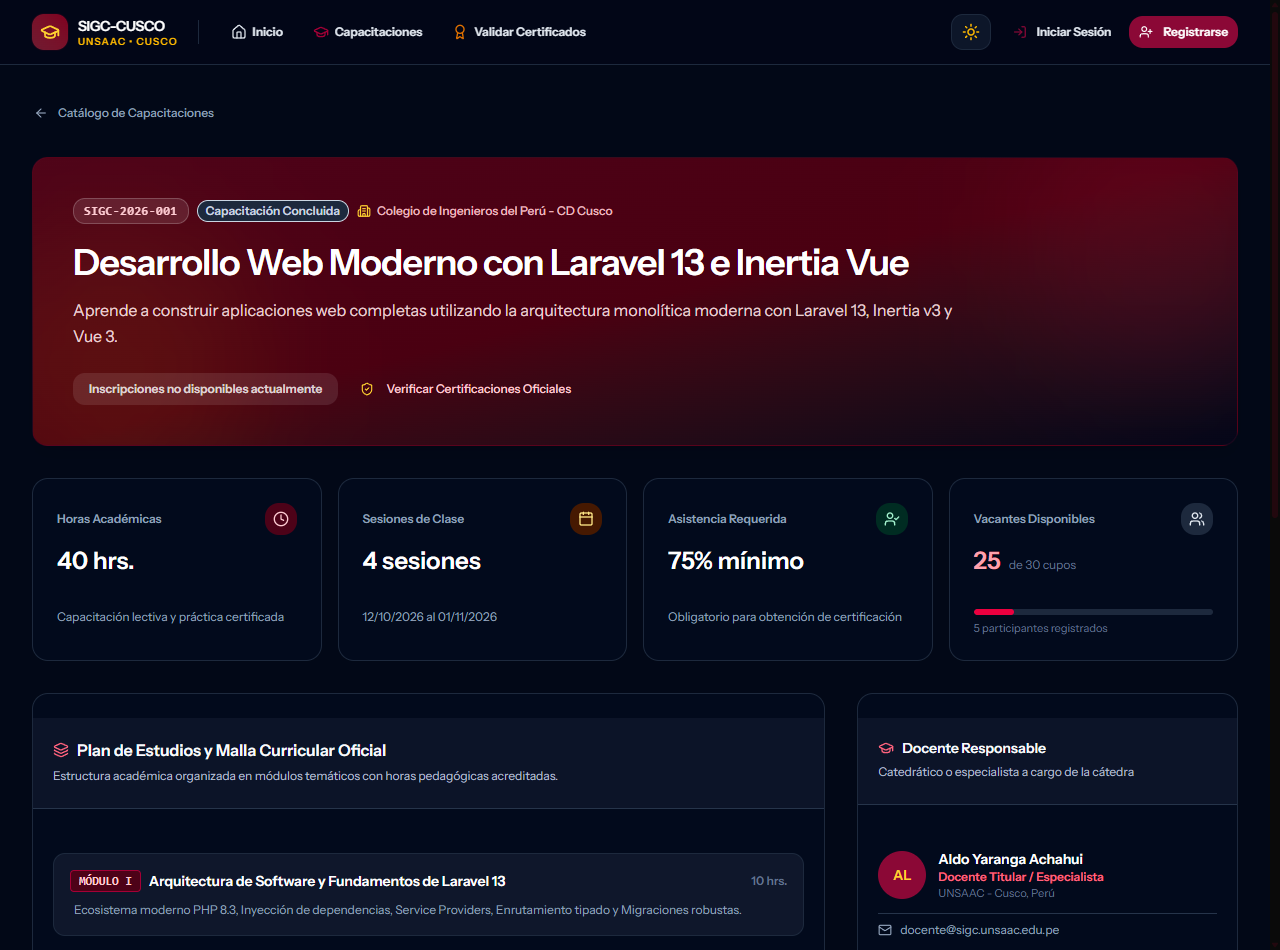
\includegraphics[width=0.94\textwidth]{sigc_real_course_detail.png}
    \caption{Ficha Detallada del Curso: Cronograma, ponente asignado, vacantes restantes y auto-matrícula.}
    \label{fig:real_course_ux}
\end{figure}

\subsection{Protocolo de Validación con Usuarios y Escala SUS}
Se aplicó una prueba de usabilidad estructurada con seis usuarios representativos de la comunidad universitaria, evaluando las interacciones críticas de administración, asistencia, cierre de actas y validación documental en el software en ejecución (\texttt{localhost:8000}).

\begin{figure}[H]
    \centering
    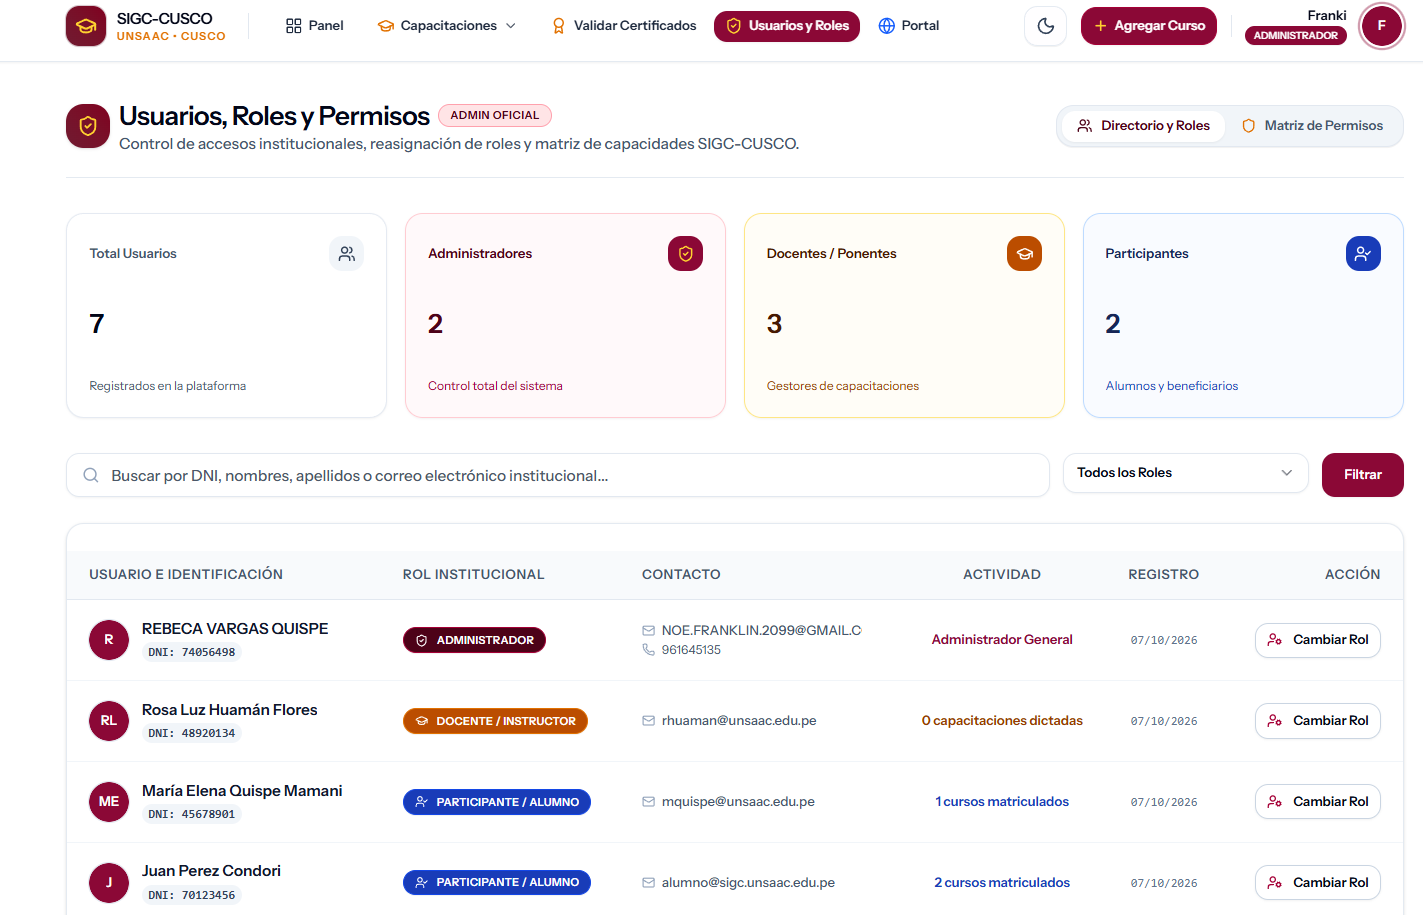
\includegraphics[width=0.94\textwidth]{evaluacion_sus_usuarios.png}
    \caption{Instrumento de Evaluación y Resultados de Usabilidad con Usuarios del Sistema SIGC-CUSCO.}
    \label{fig:evaluacion_sus_real}
\end{figure}

\begin{figure}[H]
    \centering
    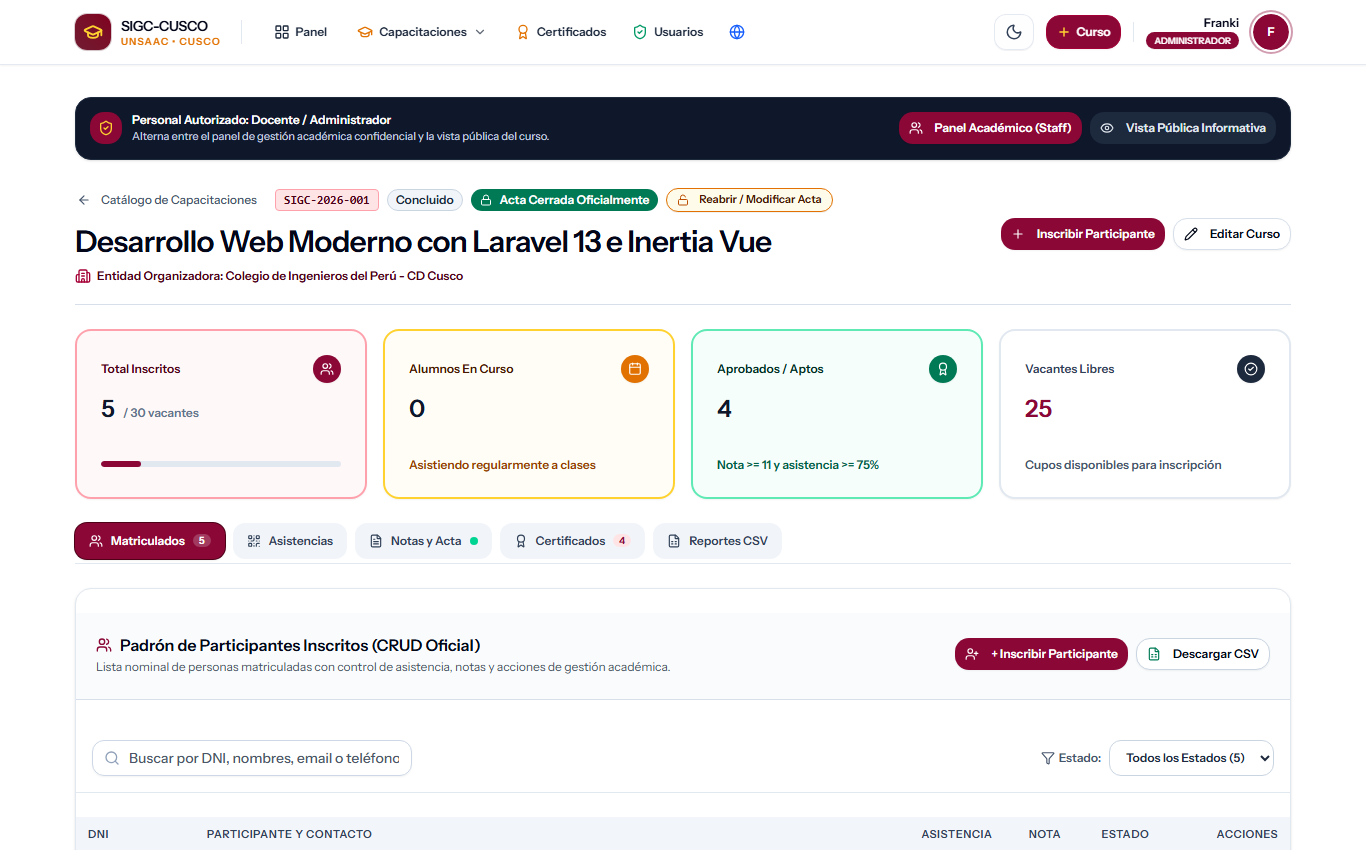
\includegraphics[width=0.94\textwidth]{sigc_gestion_academica_curso.png}
    \caption{Entorno de Validación con Usuarios: Módulo Académico del Curso con Registro de Asistencia, Evaluaciones y Emisión Masiva de Diplomas.}
    \label{fig:real_gestion_validacion}
\end{figure}

\begin{table}[H]
\centering
\small
\begin{tabularx}{\textwidth}{l P{5.0cm} P{3.5cm} Y}
\toprule
\textbf{Tarea} & \textbf{Acción Evaluada} & \textbf{Criterio de Aceptación} & \textbf{Resultado Obtenido} \\
\midrule
\textbf{T1} & Búsqueda de curso e inscripción por DNI & Tiempo de ejecución $< 30$ s & Media de 13.8 s (100\% éxito). \\
\textbf{T2} & Comprensión de alertas e inasistencias & Identificación inmediata & 100\% comprensión cromática. \\
\textbf{T3} & Verificación pública de diploma por código & Validación en 1 interacción & 100\% validado sin asistencia externa. \\
\bottomrule
\end{tabularx}
\caption{Resultados del protocolo de evaluación de usabilidad.}
\label{tab:protocolo_ux}
\end{table}

\paragraph{Puntaje Obtenido en la Escala SUS (System Usability Scale):}
La evaluación consolidada arrojó un promedio de \textbf{86.5 / 100 puntos}, correspondiente al nivel \textbf{Grado A (Excelente Usabilidad)}, validando la ergonomía cognitiva, la claridad de los componentes de interacción y la eficiencia del diseño propuesto frente a usuarios finales.
